\chapter{Optimal defence and attack strategies}
\label{chapter:Nash}
%\documentclass[10pt]{article}
%\begin{document}

%%%%%%%%%%%%%%%%%%%%%%%%%%%%%%%%%%%%%%%%%%%%%%%%%%%%%%%%%%
%%%%%			Introduction Chapter 1				%%%%%%
%%%%%												%%%%%%
%%%%%												%%%%%%
%%%%%%%%%%%%%%%%%%%%%%%%%%%%%%%%%%%%%%%%%%%%%%%%%%%%%%%%%%

%TODO-- rechtstreeks uit FlipIt paper --\\

In this chapter we are interested in finding the optimal defence and attack strategies. Ultimately, the optimal strategies can allow the determination of the Nash equilibria of the game. \\

%First the optimal functions are derived from the formulas in the previous chapter. From these piecewise functions we can derive the Nash equilibria. \\

Nash equilibria are points with the property that neither player benefits by deviating in isolation from the equilibrium. We can compute Nash equilibria for the periodic game as an intersection point of curves $opt_{D}$ and $opt_{A}$. 
\\
%As a second step, we are interested in finding Nash equilibria, points
%for which neither player will increase his benefit by changing his rate of play. 
More formally, a Nash equilibrium for the periodic game is a point $(\delta_{D}^{*},\delta_{A}^{*})$ such that
the defender's benefit $\beta_{D}(\delta_{D},\delta_{A}^{*}) $is maximized at $\delta_{D}= \delta_{D}^{*}$ and the attacker's benefit
$\beta_{A}(\delta_{D}^{*},\delta_{A}) $ is maximized at $\delta_{A}= \delta_{A}^{*}$.
To begin with, some useful notation. We denote by $opt_{D}(\delta_{A}$) the set of values (rates
of play $\delta_{D}$) that optimize the benefit of the defender for a fixed rate of play $\delta_{A}$ of the
attacker. Similarly, we denote by $opt_{D}(\delta_{D}$) the set of values (rates of play $\delta_{A}$) that optimize
the benefit of the attacker for a fixed rate of play $\delta_{D}$ of the defender. \\


% Fig \todo{fig} shows all the cases.\\
%\begin{figure}[hbtp]
%\centering
%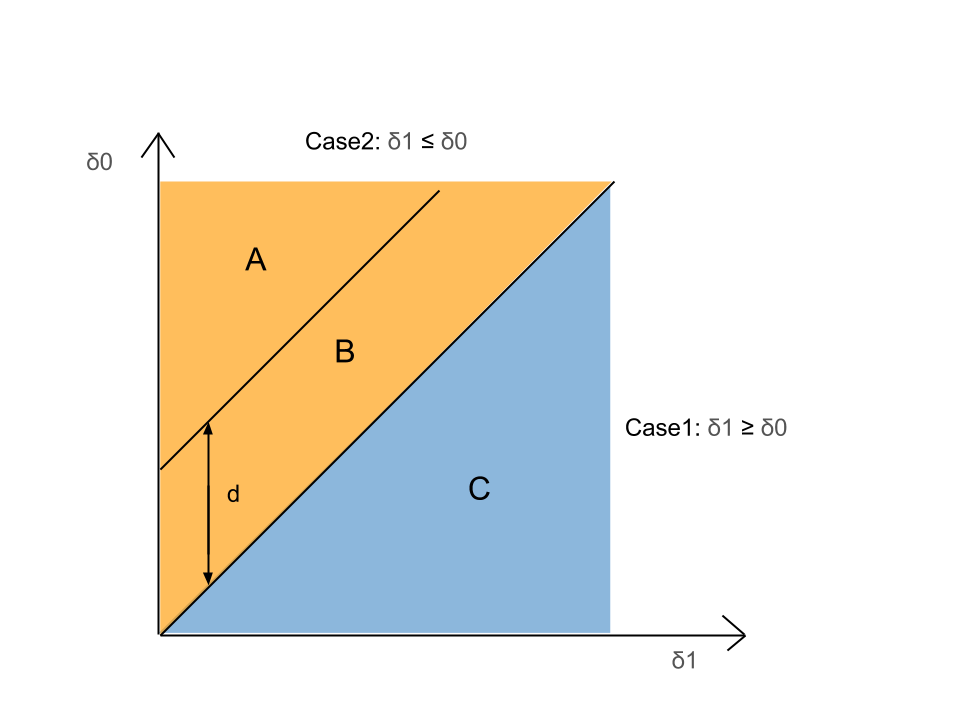
\includegraphics[scale=0.4]{Images/bestresp.png}
%\caption{This figure shows the all the cases with their subcategories. 'A' stands for Case 2.A: $\delta_{D} \geq d+\delta_{A} \geq \delta_{A}$ and 'B' stands for Case 2.B: $d+\delta_{A} \geq \delta_{D} \geq  \delta_{A} $ }
%\label{grafiekbestr}
%\end{figure}

\section{Determining the piecewise functions $opt_{D}(\delta_{A})$}

To determine $opt_{D}(\delta_{A})$ we need to compute the derivative of  $\beta_{D}(\delta_{D},\delta_{A}) $ for a fixed $\delta_{A}$.
 We consider three cases for each piece of the piecewise function of $\beta_{D}$.
 
 
\subsection*{Case A: $\delta_{D} \leq d$}

The benefit formula obtained in the previous chapter is as follows:
\begin{equation}
\beta_{D}(\delta_{D},\delta_{A}) = 1 - \dfrac{k_{D}}{\delta_{D}}
\end{equation}


The function is of the type $1-1/x$, see figure \ref{1x}. The root of the benefit function  and the root of the first derivative are as follows:
\begin{equation}
\beta_{D}(\delta_{D},\delta_{A}) =0  ~~~~~~ =>~~~~~~\delta_{D} = k_{D} \\
\end{equation}
\begin{equation}
\dfrac{\partial \beta_{D}(\delta_{D},\delta_{A})}{\partial \delta_{D}} =0 ~~~~~~ =>~~~~~~ k_{D} = 0
\end{equation}

\begin{figure}[hbtp]
\centering
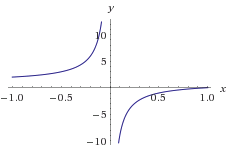
\includegraphics[scale=1]{Images/1x.png}
\caption{function of type $1-1/x$}
\label{1x}
\end{figure}

This means that if $\delta_{D} < k_{D}$  the function is negative and the defender will therefore not play, if $\delta_{D} > k_{D}$ the function is positive. If $k_{D} < 0$ the function will decrease and the defender will again not play (cost cannot be negative).  Assuming that costs are always non-negative $k_{D} > 0$, the function will increase, meaning that the slower the defender plays, the larger the benefit.



\subsection*{Case B: $ d \leq\delta_{D} \leq \delta_{A} + d$}
The defender's benefit formula obtained in the previous chapter in this case is as follows:
\begin{equation*}
\beta_{D}(\delta_{D},\delta_{A}) = 1 - \dfrac{\delta_{D}}{2\delta_{A}} - \dfrac{d^{2}}{2\delta_{D}\delta_{A}} + \dfrac{d}{\delta_{A}}  - \dfrac{k_{D}}{\delta_{D}}
\end{equation*}

To know if the function decreases or increases we take the partial derivative of this formula for a fixed $\delta_{A}$:
\begin{equation*}\label{formdelta}
\frac{\partial \beta_{D}(\delta_{D},\delta_{A})}{\partial \delta_{D}} = - \dfrac{1}{2\delta_{A}} + \dfrac{k_{D}}{\delta_{D}^{2}} + \dfrac{d^{2}}{2\delta_{D}^{2}\delta_{A}}
\end{equation*}
 
The stationary points (maximum, minimum) can be found by setting the first derivative equal to zero and finding the roots of the resulting equation:
\begin{equation*}
\frac{\partial \beta_{D}(\delta_{D},\delta_{A})}{\partial \delta_{D}} =0 ~~~~~~ =>~~~~~~ \delta_{D} = \sqrt{2\delta_{A}k_{D} + d^{2}}
\end{equation*}

Given the sign of the coefficient of $\delta_{D}^{2}$, this
leads to the following deduction: The function increases on $[0, \sqrt{2\delta_{A}k_{D} + d^{2}}]$ and is decreasing on $[\sqrt{2\delta_{A}k_{D} + d^{2}}, \infty]$. So we have a maximum at $\delta_{D} = min \{ \delta_{A} +d, \sqrt{2\delta_{A}k_{D} + d^{2}} \} $ and $\delta_{D}$ has to be larger than $d$. Taking the minimum of the two values is needed because $\delta_{D}$ cannot be larger than $\delta_{A} +d$. \\
~~\\


\subsection*{Case C: $\delta_{D} \geq d+\delta_{A} $ }

The benefit formula for the defender obtained in the previous chapter in this case is as follows:
\begin{equation*}
\beta_{D}(\delta_{D},\delta_{A})= \dfrac{\delta_{A}}{2\delta_{D}} + \dfrac{d}{\delta_{D}} - \dfrac{k_{D}}{\delta_{D}} = \dfrac{\delta_{A} + 2 (d-k_{D})}{2\delta_{D}}
\end{equation*}

Given that $\delta_{D}$ is always positive, the benefit function can be either increasing or decreasing depending on the numerator of the above fraction. \\

For $\delta_{A} + 2(d-k_{D}) > 0$ the benefit will be always positive but decreasing, see figure \ref{ShapeUp}. 
The defender will always play as fast as he can if $\delta_{A} + 2(d-k_{D}) > 0$ for $k_{D} < d$ or $k_{D} > d$ because $\delta_{A}$ will be positive in either case. There is an edge case if $d=k_{D}$, which results in a benefit of $\beta_{D}(\delta_{D},\delta_{A})= \dfrac{\delta_{A}}{2\delta_{D}}$. \\
\begin{figure}
\centering
\includegraphics[scale=0.5]{Images/ShapesUp.png} 
\caption{The benefit function is of the shape of 1/x and is always decreasing and if $\delta_{A} + 2(d-k_{D}) > 0$. }
\label{ShapeUp}
\end{figure}

For $\delta_{A} + 2(d-k_{D}) < 0$, the benefit will always be increasing but negative so the defender will not play. See figure \ref{ShapeDown}.  \\

\begin{figure}
\centering
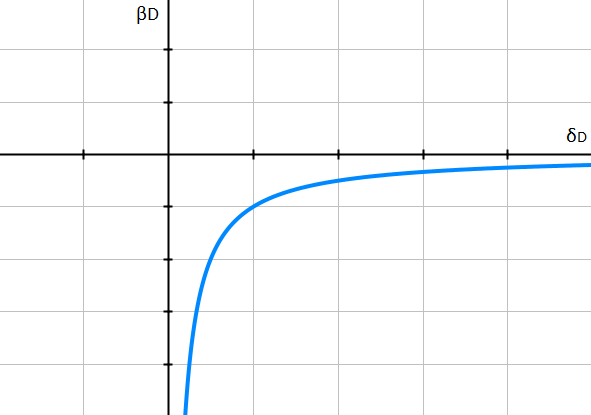
\includegraphics[scale=0.5]{Images/ShapeDown.png} 
\caption{The benefit function is of the shape of -1/x and is always increasing and if $\delta_{A} + 2(d-k_{D}) < 0$.}
\label{ShapeDown}
\end{figure}
%The derivative of the above formula for a fixed $\delta_{A}$ results in the following:
%\begin{equation*}
%\frac{\partial \beta_{D}(\delta_{D},\delta_{A})}{\partial \delta_{D}} = -\dfrac{\delta_{A}}{2\delta_{D}^{2}} - \dfrac{d}{\delta_{D}^{2}} + \dfrac{k_{D}}{\delta_{D}^{2}}
%\end{equation*}
%The obtain the stationary points the first derivative is set equal to zero and the roots of the resulting equation are found:
%\begin{equation*}
%\frac{\partial \beta_{D}(\delta_{D},\delta_{A})}{\partial \delta_{D}} =0 ~~~~~~ =>~~~~~~ \delta_{A} = 2(k_{D}-d) = dk_{D} - 2d
%\end{equation*}
%
%This leads to the following deduction:
%\begin{description}
%\item If $k_{D} \leq d$ 
%\begin{description}
% \item $\beta_{D}$ will be decreasing but always positive. If we minimize $\delta_{D}$ the value of $\beta_{D}$ will be higher. 
%\end{description}
%\item If $k_{D} > d$ 
%\begin{description}
%\item if $ \delta_{A} > 2(k_{D} -d)$, \\
%$\beta_{D}$ will be decreasing but always positive. If we minimize $\delta_{D}$ the value of $\beta_{D}$ will be higher. 
%\item if  $\delta_{A} = 2(k_{D} -d)$, \\
%the benefit of the defender will be $\beta_{D}=0$.
%\item if $\delta_{A} < 2(k_{D} -d)$, \\
%$\beta_{D}$ will be increasing but always negative. In this case the defender will not play. 
%\end{description}
%\end{description}
~~\\

%\subsection*{Case 2.B: $d+\delta_{A} \geq \delta_{D} \geq  \delta_{A} $} 
%
%The benefit formula obtained in the previous chapter  (formula \ref{benfcase2b:defender}) for the defender in this case is as follows:
%\begin{equation*}
%\beta_{D}(\delta_{D},\delta_{A}) = \dfrac{\delta_{A}}{2\delta_{D}} + \dfrac{d}{\delta_{D}} - \dfrac{k_{D}}{\delta_{D}} - \dfrac{(d-(\delta_{D} - \delta_{A}))^{2}}{2\delta_{D}\delta_{A}}
%\end{equation*}
%
%The derivative of the above formula for a fixed $\delta_{A}$ results in the following:
%\begin{equation*}
%\beta_{D}(\delta_{D},\delta_{A}) =  - \dfrac{1}{2\delta_{A}} + \dfrac{k_{D}}{\delta_{D}^{2}} + \dfrac{d^{2}}{2\delta_{D}^{2}\delta_{A}}
%\end{equation*}
%
%
%The stationary points (maximum, minimum) can be found by setting the first derivative equal to zero and finding the roots of the resulting equation:
%
%\begin{equation*}
%\frac{\partial \beta_{D}(\delta_{D},\delta_{A})}{\partial \delta_{D}} =0 ~~~~~~ =>~~~~~~ \delta_{D} = \sqrt{2\delta_{A}k_{D} + d^{2}}
%\end{equation*}
%
%
%For case 2.B this leads to the following deduction, which results in the same formula as for case 1 but with a small difference for the value of $\delta_{D}$: The function increases on $[0, \sqrt{2\delta_{A}k_{D} + d^{2}}]$ and is decreasing on $[\sqrt{2\delta_{A}k_{D} + d^{2}}, \infty]$. Because $\delta_{D} \geq \delta_{A}$ there is a maximum on $\delta_{D} = maximum \{ \delta_{A}, \sqrt{2\delta_{A}k_{D} + d^{2}} \} $ or because $d+\delta_{A} \geq \delta_{D}$ there is also on $\delta_{D} = minimum \{ \delta_{A}+d, \sqrt{2\delta_{A}k_{D} + d^{2}} \} $. %-Remark- \todo{beter uitschrijven, deltaD moet tussen die twee waarden liggen}\\

\section{Best responses of $\delta_{D}$}
The optimum functions will be piecewise functions. We distinguish six cases for different values of $\delta_{A}$ depending on the values of $k_{D}$ and $d$. 
%We point out that $\delta_{A}$ and $\delta_{D}$ are positive rates. 


\subsection*{$\delta_{A} < 2(k_{D} - d)$}
From case C above, it follows that if $\delta_{A} < 2(k_{D} - d)$ the benefit is increasing but it will always be non-positive. The defender will try not to play ($\delta_{D}= \infty$). 

%From case C it follows that from interval $[2(k_{D} -d), \sqrt{2k_{D}\delta_{A} + d^{2}}]$  (because for case 2 $\delta_{D} \geq \delta_{A}$), that the benefit is increasing.  The maximum of case 2.a and the maximum of case 2.b can be brought together. It follows that the optimal benefit is achieved at the $\delta_{D}=minimum[\delta_{A} + d, \sqrt{2k_{D}\delta_{A} + d^{2}}]$, which is $\delta_{D}=\sqrt{2k_{D}\delta_{A} + d^{2}}$. But because of case 2.a, the defender's maximum benefit is not to play at all.

\subsection*{$\delta_{A} = 2(k_{D} - d)$}
For case C, $\beta_{D}(\delta_{D}, \delta_{A})=0$ for  all $\delta_{D} \in [\sqrt{2k_{D}\delta_{A} + d^{2}}, \infty]$. For case B, the benefit is increasing in the interval $[\delta_{A},\sqrt{2k_{D}\delta_{A} + d^{2}}]$. If we put both cases back together, we get a maximum at $\sqrt{2k_{D}\delta_{A} + d^{2}}$. So in this case the defender's maximum benefit is achieved for any $\delta_{D}$ in $[\sqrt{2k_{D}\delta_{A} + d^{2}}, \infty]$ with value 0.

\subsection*{$\delta_{A} > 2(k_{D} - d)$ }
For case C, it follows that the benefit is decreasing but positive. So the defender will try to play as fast as possible ($\delta_{D} \rightarrow 0$). For case B it is increasing in the interval $[ 0,\sqrt{2k_{D}\delta_{A} + d^{2}}]$. It follows that the defender's maximum benefit is achieved for $\delta_{D} = \sqrt{2k_{D}\delta_{A} + d^{2}} $  \\


~~\\
From this analyses we can compute $opt_{D}(\delta_{A})$ : \\

 \begin{displaymath}
  opt_{D}(\delta_{A}) = \left\{
     \begin{array}{lr}
          \infty , & \delta_{A} < 2(k_{D} - d)\\
      \left[ \sqrt{2k_{D}\delta_{A} + d^{2}},\infty\right] , & \delta_{A} = 2(k_{D} - d) \\
      \sqrt{2k_{D}\delta_{A} + d^{2}}, & \delta_{A} > 2(k_{D} - d)
     \end{array}
   \right.
\end{displaymath}

~~\\


\subsection*{Edge cases:}

\subsection*{$\delta_{A}=0$ and $k_{D}=0$}
If $\delta_{A}=0$ it means that the attacker is playing as fast as possible. For the defender it does not cost anything to flip, because $k_{D}=0$. We know that if $\delta_{D} \leq d$ the defender always has a benefit of 1. This means that for this case the defender will play with a rate $\delta_{D} \in [0,d]$.

-- ofwel volgende uitleg--- \\
If $k_{D}=0$ it means that every flip of the defender is free. So for the cost it does not matter for the defender if he plays faster or slower. $\delta_{A}=0$ means that the attacker will play as fast as he can.  
\begin{itemize}
\item if $d=0$, if we look at $opt_{D}(\delta_{A})$ it means that we are in the second piece. The defender will play with a rate of $[0,\infty]$. 
\item if $d >0$, we have to look at the third piece of  $opt_{D}(\delta_{A})$ . Here it follows that the defender has to play with a rate of \textit{d}.
\end{itemize}

Combining those two leads to a rate for the defender equal to $[0,d]$. This means that the defender will never not play, which is intuitively correct if we know that the defender has no disadvantage to play because there is no cost involved.
\subsection*{$\delta_{A}=0$}
If $\delta_{A}=0$ it means that the attacker is playing as fast as possible. The defender has still a cost for every flip.
\begin{itemize}
\item if $k_{D} > d$, we look at the first piece of $opt_{D}(\delta_{A})$. It follows that the defender will not play (rate equal to $\infty$).
\item if $k_{D}=d$, corresponds to the second piece: the defender will play with a rate of $[d,\infty]$.
\item if $k_{D} < 0$, for the last case the rate of the defender corresponds to \textit{d}.
\end{itemize}
~~\\
   $  \infty \& \delta_{A}=0 ~~ \& ~~ k_{D} > d$ \\
Combining the results leads to a rate for the defender equal to $[d,\infty]$. 
\subsection*{$k_{D}=0$}
The cost of flipping for the defender is equal to zero. 

\subsection{Conclusion}
With the edge cases we can compute $opt_{D}(\delta_{A})$ : \\

 \begin{displaymath}
  opt_{D}(\delta_{A}) = \left\{
     \begin{array}{lr}
     \left[0,d\right] & \delta_{A} =0 ~~\& ~~k_{D}=0 \\
     \left[0,d\right] & k_{D}=0\\
     d & \delta_{A} =0 ~~ \& k_{D} \leq d\\
          \infty , & \delta_{A} < 2(k_{D} - d)\\
      \left[ \sqrt{2k_{D}\delta_{A} + d^{2}},\infty\right[ , & \delta_{A} = 2(k_{D} - d) \\
      \sqrt{2k_{D}\delta_{A} + d^{2}}, & \delta_{A} > 2(k_{D} - d)
     \end{array}
   \right.
\end{displaymath}
%*****************************************************************
%
% optimum functies voor beta A
%
%*********************************************************************
\section{Determining the piecewise functions $opt_{A}(\delta_{D})$}
%To start with we only consider the case where $d < \delta_{D}$, because if $d > \delta_{D}$ the benefit of the defender \todo{nakijken, def of att} is always 1. \\
To determine the optimal strategy of the attacker we also need to determine $opt_{A}(\delta_{D})$ by computing the derivative of $\beta_{A}(\delta_{D},\delta_{A})$ for a fixed $\delta_{D}$. We consider the three cases of the piecewise function of $\beta_{A}$: \\


\subsection*{Case A: $\delta_{D} \leq d$}

The benefit formula obtained in the previous chapter is as follows:
\begin{equation}
\beta_{A}(\delta_{D},\delta_{A}) =  - \dfrac{k_{A}}{\delta_{A}}
\end{equation}


The function is of the type $-1/x$, see figure \ref{1xx}. The root of the benefit function is as follows:
\begin{equation}
\beta_{A}(\delta_{D},\delta_{A}) =0  ~~~~~~ =>~~~~~~k_{D} = 0 \\
\end{equation}


\begin{figure}[hbtp]
\centering
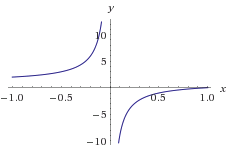
\includegraphics[scale=1]{Images/1x.png}
\caption{function of type $-1/x$}
\label{1xx}
\end{figure}

This means that if $k_{A} < 0$ the benefit function is positive and decreasing but $k_{D}$ cannot be negative so the attacker will not play. If $k_{A} > 0$ the function will be negative but always increasing.



\subsection*{Case B: $d \leq \delta_{D} \geq \delta_{A} + d$}

The benefit formula obtained in the previous chapter \ref{Benfcase1:attacker} for this case is as follows:
\begin{equation*}
\beta_{A}(\delta_{D},\delta_{A}) =\dfrac{\delta_{D}}{2\delta_{A}} - \dfrac{k_{A}}{\delta_{A}} + \dfrac{d^{2}}{2\delta_{D}\delta_{A}} - \dfrac{d}{\delta_{A}}
\end{equation*}
The derivative for a fixed $\delta_{D}$ is as follows:
\begin{equation*}
\dfrac{\partial \beta_{A}(\delta_{D},\delta_{A})}{\partial \delta_{A}} = -\dfrac{\delta_{D}}{2\delta_{A}^{2}} + \dfrac{k_{A}}{\delta_{A}^{2}} - \dfrac{d^{2}}{2\delta_{D}\delta_{A}^{2}} + \dfrac{d}{\delta_{A}^{2}} = \dfrac{-\delta_{D}^{2} - d^{2} + 2\delta_{D}d + 2\delta_{D}k_{A}}{2\delta_{A}^{2}\delta_{D}}
\end{equation*}
The stationary points (maximum, minimum) can be found by setting the first derivative equal to zero and finding the roots of the resulting equation:
\begin{equation*}
\frac{\partial \beta_{A}(\delta_{D},\delta_{A})}{\partial \delta_{D}} =0 ~~~~~~ =>~~~~~~  \delta_{D}= \dfrac{(\delta_{D}-d)^{2}}{2k_{A}}
\end{equation*}

It follows that $\beta_{A}(\delta_{D},\cdot)$ is increasing and non-positive if $\delta_{D}> \dfrac{(\delta_{D}-d)^{2}}{2k_{A}}$ and decreasing and positive if $\delta_{D} < \dfrac{(\delta_{D}-d)^{2}}{2k_{A}}$  \\

\subsection*{Case B: $\delta_{D} \geq d+\delta_{A} \geq \delta_{A} $ }
The benefit formula obtained from the previous chapter \ref{benfcase2a:attacker} for this case is as follows:
\begin{equation*}
\beta_{A}(\delta_{D},\delta_{A}) =1- \dfrac{\delta_{A}}{2\delta_{D}} - \dfrac{k_{A}}{\delta_{A}} - \dfrac{d}{\delta_{D}}
\end{equation*}
The derivative for a fixed $\delta_{D}$ is as follows:
\begin{equation*}
\dfrac{\partial \beta_{A}(\delta_{D},\delta_{A})}{\partial \delta_{A}} = \dfrac{-1}{2\delta_{D}} + \dfrac{k_{A}}{\delta_{A}^{2}}
\end{equation*}
The stationary points (maximum, minimum) can be found by setting the first derivative equal to zero and finding the roots of the resulting equation:
\begin{equation*}
\frac{\partial \beta_{A}(\delta_{D},\delta_{A})}{\partial \delta_{D}} =0 ~~~~~~ =>~~~~~~ \delta_{A} = \sqrt{2\delta_{D}k_{A}}
\end{equation*}
It follows that $\beta_{A}(\delta_{D},\cdot)$ is increasing on $[0,\sqrt{2k_{A}\delta_{D}}]$ and decreasing on $[\sqrt{2k_{A}\delta_{D}}, \infty]$ and thus has a maximum on $\delta_{A} = minimum \{\delta_{D} -d, \sqrt{2k_{A}\delta_{D}} \} $. The minimum between $\delta_{D}-d$ and $ \sqrt{2k_{A}\delta_{D}}$ is needed because $\delta_{A} $ cannot exceed $\delta_{D}-d$ in this case. \\

%\subsection*{Case 2.B: $d+\delta_{A} \geq \delta_{D} \geq  \delta_{A} $} 
%
%The benefit formula obtained from the previous chapter \ref{benfcase2b:attacker} for this case is as follows: 
%\begin{equation*}
%\beta_{A}(\delta_{D},\delta_{A}) = 1 - \dfrac{•}{•}\delta_{A}}{2\delta_{D}} - \dfrac{d}{\delta_{A}} - \dfrac{k_{A}}{\delta_{A}} + \dfrac{(d-(\delta_{D}-\delta_{A})^{2}}{2\delta_{D}\delta_{A}} 
%\end{equation*}
%The derivative for a fixed $\delta_{D}$ is as follows:
%\begin{equation*}
%\dfrac{\partial \beta_{A}(\delta_{D},\delta_{A})}{\partial \delta_{A}} = -\dfrac{\delta_{D}}{2\delta_{A}^{2}} + \dfrac{k_{A}}{\delta_{A}^{2}} - \dfrac{d^{2}}{2\delta_{D}\delta_{A}^{2}} + \dfrac{d}{\delta_{A}^{2}}
%\end{equation*}
%The stationary points (maximum, minimum) can be found by setting the first derivative equal to zero and finding the roots of the resulting equation:
%\begin{equation*}
%\frac{\partial \beta_{A}(\delta_{D},\delta_{A})}{\partial \delta_{D}} =0 ~~~~~~ =>~~~~~~ \delta_{D}= \dfrac{(\delta_{D}-d)^{2}}{2k_{A}}
%\end{equation*}
%
%
%It follows that $\beta_{A}(\delta_{D},\cdot)$ is increasing and non-positif if $\delta_{D} > \dfrac{(\delta_{D}-d)^{2}}{2k_{A}}$ and decreasing and positive if $\delta_{D} < \dfrac{(\delta_{D}-d)^{2}}{2k_{A}}$. This is the same result as in case 1.\\


\section{Best responses of $\delta_{A}$}
The optimum functions will be piecewise functions. We distinguish three cases for different values of $\delta_{D}$ regarding $d$ and $k_{A}$. 


For this term $\dfrac{(\delta_{D}-d)^{2}}{2k_{A}} $ , $d$ has to be bigger than  $\delta_{D}$ because the cost $\delta_{D}$ cannot be negative. This was an assumption that was already made, because the benefit of the defender will always be 1 if $d$ is bigger than  $\delta_{D}$.

\subsubsection*{$\delta_{D} < \dfrac{(\delta_{D}-d)^{2}}{2k_{A}}$} 
From case 1 and case 2.b above, it follows that the benefit is decreasing but positive, which means that the attacker will play as fast as he can. For case 2.a  $\delta_{D} \geq \delta_{A}$ is increasing. It follows that for this case the attacker's maximum benefit is achieved for $\delta_{A} = \sqrt{d k_{A}\delta_{D}}$.
. In this case the attacker's maximum benefit is reached at $\delta_{A} = \delta_{A} = \sqrt{dk_{A}\delta_{D}}$  .
\subsubsection*{$\delta_{D} = \dfrac{(\delta_{D}-d)^{2}}{2k_{A}}$} 
The benefit $\beta_{A}(\delta_{D},\delta_{A})=0$ for case 1 and case 2.b for all $\delta_{D}$ in $[0, \infty [$. For case 2.a it follows that the benefit is increasing. The attacker's maximum benefit is achieved at any $\delta_{A} $ in 
\subsubsection*{$\delta_{D} > \dfrac{(\delta_{D}-d)^{2}}{2k_{A}}$} 
For case 1 and case 2.b the benefit is increasing but non-positive. This means that the attacker won't play ($\delta_{A} = \infty$). 
\\
~~\\
From this analyses we can compute $opt_{A}(\delta_{D})$ : 

 \begin{displaymath}
  opt_{A}(\delta_{D}) = \left\{
     \begin{array}{lr}
            \infty & \delta_{D} < \dfrac{(\delta_{D}-d)^{2}}{2k_{A}} \\
       \left[ \sqrt{d k_{A}\delta_{D}}, \infty\right],  & \delta_{D} = \dfrac{(\delta_{D}-d)^{2}}{2k_{A}} \\
       \sqrt{d k_{A}\delta_{D}}, & \delta_{D} > \dfrac{(\delta_{D}-d)^{2}}{2k_{A}}
     \end{array}
   \right.
\end{displaymath}
\\

\subsection*{Edge cases:}

\subsection*{$\delta_{D}=0$ and $k_{A}=0$}
If $\delta_{D}=0$, looking at the benefit formula of the attacker, it follows that the period of the defender will always be equal or smaller than the delay. The delay cannot be negative. So from case $\delta_{D} \leq d$ it follows that the attacker will always have a benefit equal to zero, because $k_{A}=0$. For the attacker it does not matter what he plays. The benefit will always be the same. The optimal strategy in this case for the attacker will be playing at a rate $\delta_{A} \in [0,\infty ]$.

\subsection*{$k_{A}=0$}
If the cost of playing for the attacker is zero, the attacker can play as fast as he can.  If $\delta_{D} \leq d$, looking at the benefit formula for the attacker, it does not matter what the attacker does, his benefit will always be zero. He will play with a rate $\delta_{A} \in [0,\infty ]$.  We can merge this with the previous case where $\delta_{D}=0$ and $k_{A}=0$.  If $\delta_{D} > d$, the attacker will play. He will play with a rate of $\delta_{A} \in [0, \delta_{D} - d ]$. 
\subsection*{$\delta_{D}=0$}
If $\delta_{D}=0$ it follows from the case $\delta_{D} \leq d$ that the attacker will always have a negative benefit, unless the cost is zero. If the cost is zero we have again the case of $\delta_{D}=0$ and $k_{A}=0$. But if the cost is non-zero, the optimal strategy of the defender is not moving at all. 

\subsection{Conclusion}
With the edge cases we can compute $opt_{A}(\delta_{D})$ : \\

 \begin{displaymath}
  opt_{A}(\delta_{D}) = \left\{
     \begin{array}{lr}
     \infty & \delta_{D} = 0 \\
     \left[0,\infty\right] & \delta_{D} \leq d ~~\& ~~k_{A}=0 \\
          \left[0,\delta_{D} - d\right] & \delta_{D} > d ~~\& ~~k_{A}=0 \\
                 \infty & \delta_{D} < \dfrac{(\delta_{D}-d)^{2}}{2k_{A}} \\
       \left[ \sqrt{d k_{A}\delta_{D}}, \infty\right],  & \delta_{D} = \dfrac{(\delta_{D}-d)^{2}}{2k_{A}} \\
       \sqrt{d k_{A}\delta_{D}}, & \delta_{D} > \dfrac{(\delta_{D}-d)^{2}}{2k_{A}}
     \end{array}
   \right.
\end{displaymath}
\\

\section{Conclusion}
The Nash Equilibria can be found as the intersection points of the piecewise functions $opt_{A}(\delta_{D})$ and $opt_{D}(\delta_{A})$. For this we have to compare the function in terms of the relationship of the players move cost. We distinguish three cases: $k_{A} < k_{D} , ~k_{A} > k_{D} $ and $k_{A} = k_{D}$. 
